\section{The population section\label{sec:population-section}}

The population section\index{Population section} defines the model of the movement and population dynamics. It describes the model structure (both the spatial and population structure), defines the population and movement processes (for example, recruitment, migration, and mortality), defines the layers (the known attributes of each spatial cell), selectivities, and model parameters.

The population, at any point in time, is described by the \emph{state}, which comprises of the \emph{partition} and any \emph{derived quantities}. The partition is comprised of the spatial structure, and within each spatial location, the population structure. 

The spatial structure of \SPM\ is represented by an $n \times m$ grid, with rows $i=1 \dots n$ and columns $j=1 \ldots m$. Each cell of this matrix records the population structure at that point in space and is represented by an $k \times l$ rectangular matrix (with categories $k=1 \ldots k$ and ages $l=age_{min} \ldots age_{max}$. Hence we can describe any spatial and population element of the model as element$(i,j,k,l)$. 

\subsection{Spatial structure}

\SPM\ implements two spatial structures, one derived from a grid of \emph{square} cells \textemdash the default (Figure \ref{fig:SquareSpatialStructure}) and the other derived from a grid of north-south orientated \emph{hexagons} (Figure \ref{fig:HexagonSpatialStructure}). 

The dimensions of the spatial grid are user defined but must be at least a $1 \times 1$ grid (i.e., a single spatial cell). Associated with the spatial structure is the one compulsory layer (see Section \ref{sec:layers}), the \emph{base layer}. This defines the locations where the population can and cannot potentially be present (e.g., in a marine model, the locations associated with the sea and not land) as values within the base layer that are greater than zero. There must be at least one cell in the spatial grid where the population can be present. In addition, the base layer also defines the relative \emph{area} of each spatial cell, as used for density calculations within \SPM.

\begin{figure}[htp]
 \centering
  \resizebox{\textwidth}{!}{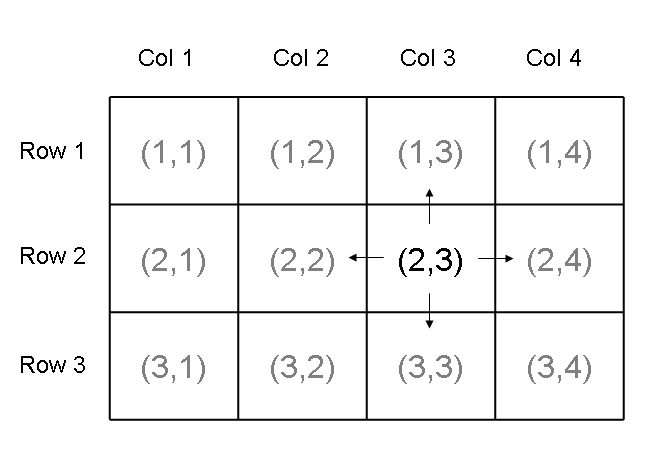
\includegraphics[width=\textwidth]{Figures/SquareStructure}}
  \caption{An illustration of the \emph{square} spatial structure}
  \label{fig:SquareSpatialStructure}
\end{figure}

\begin{figure}[htp]
 \centering
  \resizebox{\textwidth}{!}{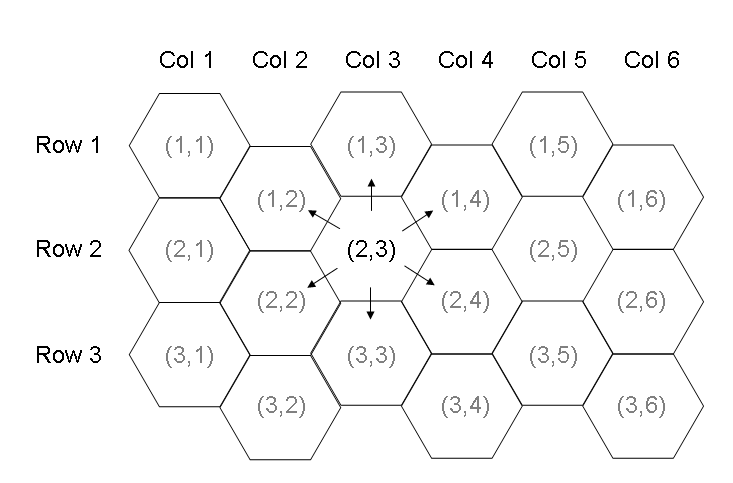
\includegraphics[width=\textwidth]{Figures/HexagonStructure}}
  \caption{An illustration of the \emph{hexagon} spatial structure}
  \label{fig:HexagonSpatialStructure}
\end{figure}

Models can be implemented as a grid based on either squares or hexagons, but not both. This choice effects the location of neighbours (for adjacent movements) and the distance between cells (for preference based movements). Distance between cells is determined as the euclidean distance between cell centres, modified by an arbitrary scalar. 

Hence, the definition of the spatial structure includes;
\begin{itemize}
\item The type of spatial grid and its dimensions, $n_{rows}$ and $m_{cols}$
\item The label of a numeric layer to be used as the base layer (defining the locations where the population can be present as well as the area of each cell)
\item the length (distance) of a side of the grid (either a square or hexagon) to be used as the scaler for distance calculations
\end{itemize}

\subsection{Population structure}

The population structure in \SPM\ is represented by a matrix containing an arbitrary number of user defined categories (rows), and an arbitrary age range (columns). Hence, each spatial cell has a population state described as $n_{categories} \times n_{ages}$ rectangular matrix with categories $k=1 \ldots n_{categories}$ and ages $l=age_{min} \ldots age_{max}$. 

The names and number of categories are user defined, but there  just be at least one category in any model. The ages are defined as a sequence from $age_{min}$ to $age_{max}$, and the last age may optionally be a plus group.

Hence, the definition of the population structure includes;
\begin{itemize}
  \item The number and labels of the categories, $k_{categories}$
  \item The minimum and maximum ages that define the ages of the model, $l_{ages}$
  \item If the last age is a plus group
\end{itemize}

\subsection{Layers\label{sec:layers}}

Layers form a key underlying concept in \SPM. They comprise of a grid of known values, with a value for every spatial cell in the model. Layers are used by processes, observations, and outputs commands to supply spatially explicit covariates and any categorical groupings required. 

Every model must define at least one layer, the base later $L_B$. A layer is defined as a $n_{rows} \times n_{cols}$ grid of values (with one exception \textemdash the distance layer, see below), where the value for each cell represents a known quantity. For example layers may represent classifications, physical attributes, or some other assumed quantity. Typically they are provided by the user as a matrix of values, although abundance and distance layers can be calculated by \SPM\ as and when required. 

Within \SPM, layers are used in three contexts:
\begin{enumerate}
\item The base layer: The base layer $L_B$ is a special layer (there must be exactly one base layer defined within the model) that defines the locations where the population can and cannot potentially be present (e.g., locations associated with the sea and not land in a marine model). Here, we define that a cell may potentially have part of the population present if every element $L_B(i,j) \ge 0$. Further, positive values of the base layer $L_B$ represent the \emph{area} represented by that spatial cell. 
\item Covariate layers: A model may have many covariate layers, and these are used as covariates of some population or movement process (e.g., the sea floor depth may be a covariate of some movement process). The values in layers used as covariates must be continuous (i.e., numeric) variables. Covariate layers must have values $\ge0$.
\item Classification layer. A model may have many classification layers, and these are used as a classification or grouping variable for aggregating data over individual spatial cells $(i,j)$, e.g., statistical areas or management areas. Such layers are typically used to aggregate the population within cells into groups so-as to allow comparison with observations. The values in layers used as classification layers must be categorical.
\end{enumerate}

Typically, layers are supplied by the user and are assumed known and constant. \SPM\ defines the following types of layer;

\begin{enumerate}
\item{Numeric layer\label{numeric-layer}}: A model may have many numeric layers, and these can be used as covariates of a population or movement process (e.g., depth may be a covariate of some movement process), and/or locations of event mortality. Numeric layers can contain only continuous (numeric) variables. Values for a numeric layer must be supplied for each cell by the user.

\item {Categorical layer\label{categorical-layer}}: A model may have many categorical layers, and these are used as a classification or grouping variable for aggregating data over individual cells, e.g., management areas. Such layers are typically used to aggregate the population within cells into groups for comparing with observations. The values in layers used as categorical layers can contain any characters (except white space), and are interpreted as categorical values. Values for a categorical layer must be supplied for each cell by the user.

\item {Distance layer}: A distance layer is one that defines the distance between any two cells. By default, \SPM\ calculates the values of the distance layer as the Euclidean distance (where the grid type is \argument{square}). Here, the distance between cell a and cell b can be defined as,
\begin{equation}
  d(a,b) = \lambda \sqrt{(x_a - x_b)^2 + (y_a - y_b)^2}
\end{equation}
where $x$ and $y$ represent the x- and y-coordinates of $a$ and $b$ respectively, and $\lambda$ is an arbitrary scaler representing the length of one side of the square. Unlike other types of layers, distance layers are not a $n_{rows} \times n_{cols}$ grid of values, but rather a matrix of dimension $(n_{rows} \times n_{cols}) \times (n_{rows} \times n_{cols})$  where the distance between each cell and every other cell is evaluated. Note that under this definition, the distance between any cell and itself is 0. 

\item{Abundance layer}: The abundance layer is the sum of the number of individuals within cell $a$ in categories $k$ and with selectivity $S_l$ at age $l$. 
\begin{equation}
  N(a) = \sum\limits_{k} \sum\limits_l S_l \ \text{element}(i,j,k,l)
\end{equation}
\SPM\ calculates the values of the layer when running the model at the point in time where the value is required.

\item {Biomass layer}: The biomass layer is the sum of the biomass of individuals within cell $a$ in categories $k$, with selectivity $S_l$ at age $l$, and mean weight $w_{kl}$
\begin{equation}
  N(a) = \sum\limits_{k} \sum\limits_l w_{k,l} S_l \ \text{element}(i,j,k,l) 
\end{equation}
\SPM\ calculates the values of the layer when running the model at the point in time where the value is required.

\item {Abundance-density layer}: The abundance density layer is the density of the number of individuals within cell $a$ with area $A_a$ in categories $k$, with selectivity $S_l$ at age $l$,
\begin{equation}
  N(a) = \frac{1}{A_a} \sum\limits_{k} \sum\limits_l S_l \ \text{element}(i,j,k,l)
\end{equation}
\SPM\ calculates the values of the layer when running the model at the point in time where the value is required.

\item {Biomass-density layer}: The biomass-density layer is the density of the biomass of individuals within cell $a$ with area $A_a$ in categories $k$, with selectivity $S_l$ at age $l$, and mean weight $w_{kl}$,
\begin{equation}
  N(a) = \frac{1}{A_a} \sum\limits_{k} \sum\limits_l w_{k,l} S_l \ \text{element}(i,j,k,l)
\end{equation}
\SPM\ calculates the values of the layer when running the model at the point in time where the value is required.

\item {Meta-layer\label{meta-layer}}: In addition to the above types of layer, \SPM\ defines a special type of layer known as a \emph{meta-layer}. The meta-layer allows individual layers (of the same type) to be indexed by year, and applied as a single layer within the model. For example, assume that we had a model where we wished to use Sea Surface Temperature (SST) as a layer, perhaps to control some movement process. The SST values for each year of the model would be defined as individual numeric layers, each with a unique label. We could then define a meta-layer that indexed the individual annual SST layers by year, and use the meta-layer as the control layer in the movement process. 
\end{enumerate}

However, there are  exceptions to this rule \textemdash layers of type biomass, quantity, and distance are calculated automatically by \SPM\ as required. For example, for the distance layer in a square grid, the distance between cell $a$ and cell $b$ is defined as proportional to $\sqrt{(x_a-x_b)^2 +(y_a-y_b)^2}$, where $x$ and $y$ represent the x- and y-coordinates of $a$ and $b$ respectively.

For the abundance layer, the abundance or biomass of a cell is simply a count of the number (or biomass) of individuals in the cell a within categories $K$, with selectivity $S$, e.g., $N(a)=\sum_k \sum_i \ \text{element}(i,j,k,l)$.

Note that \SPM\ does not `edit' or otherwise change layers, including adding or otherwise combining layers that are supplied in the input parameter files \textemdash\ except for a single case for numeric layers. In that instance, the numeric layer supplied can optionally be standardized prior to use, i.e., $L'(a)=L(a)/\max(L)$ so that $L'(a) < 1$.

\subsection{Time sequence}

The time sequence of the model is defined in three parts;
\begin{itemize}
  \item Initialisation 
  \item Run years
  \item Projection years
\end{itemize}

\subsubsection{Model initialisation}

\SPM\ initialises the initial equilibrium state as an iterative process, because a general solution that initialises complex structured movement models can be difficult to implement using analytic techniques. However, initialising via iteration for a long-lived species with complex movements can also be slow to run. In \SPM, we allow for user-defined multi-phased initialisation using iteration to allow the user to optimize models for speed. Each phase of the initialisation can involve any number of population and/or movement processes. 

The initialisation part can consist of one or more phases, with each phase occurring for at least one year. Within each phase, the processes defined for that phase are carried out, and use as the starting point for the following phase, or if it is the last phase, then the years that the model is run over. The first phase is always initialised with each element (i.e., each age and category within each spatial cell) seeded with a zero. Note that this means that recruitment processes where the numbers of recruits is based on a stock recruitment or density dependant relationship will likely fail. 

Hence, you need to define;
\begin{itemize}
  \item The initialisation phases
  \item The number of years in each phase and the processes to apply in each
\end{itemize}

\subsubsection{Model years}

Following initialisation, the model then runs over a number of user-defined years. For this part of the model, the annual cycle can be broken into separate time steps, and observations can be associated with the state of the model at the end of any time step, i.e., likelihoods for particular observations are evaluated, if required, at the end of each time step. 

Processes are carried out in the order specified within each time step, and can be the same or different to processes in other initialisation phases of the model. The run years define the years over which the model is to run and the annual cycle within each year. The model runs from the start of year \argument{initial} and runs to the end of year \argument{current}. The projection part then extends the run time up to the end of year \argument{final}. 

\begin{itemize}
  \item The time steps and the processes applied in each
  \item The initial year (i.e., the model start year)
  \item The current year (i.e., the model end year)
  \item The final year (i.e., the model projection end year)
\end{itemize}

\subsection{Processes}

Processes produce changes in the model partition, by adding, removing or moving individuals between spatial cells (movement processes), and ages or categories (population processes). These include processes such as recruitment, mortality, ageing, and movements.

An \SPM\ model can be parametrised by both population processes (for example, ageing, recruitment, and mortality), and movement processes. Population processes are those processes which modify, move or otherwise change the numbers of individuals within a spatial cell, i.e., they do not affect the spatial location of a cohort. Movement processes, on the other hand, move, shift or otherwise modify cohorts between spatial cells, but do not affect the age or category of the numbers in each cohort. 

\subsection{Population processes}

Population processes are those processes that change the population state of individuals, but retain their location. 

\subsubsection{Recruitment}

Recruitment processes are defined as  process that introduces new individuals into the model. \SPM\ implements two types of recruitment process, constant recruitment and Beverton-Holt recruitment \citep{1203}. 

In both of the recruitment process, a number of individuals are added to the partition at the age and categories specified. If more than one category is defined, then the proportions of individuals added across categories are user-defined. For example, if recruiting to categories labelled male and female, then you might set the proportions as $0.5$ and $0.5$ respectively to denote that half of the recruits recruit to the male category and the remaining half to the female category.

For each cell where cell$(i,j)$ is a member of some layer $L_R$, the  number of fish added in year $y$ is 
\begin{equation}
  \text{element}(i,j,k,l) \leftarrow \text{element}(i,j,k,l) + p_k(R_y / n)
\end{equation}

where age is the age defined as the recruitment age, $p_k$ is the proportion recruitment to category $k$ defined to have recruitment, and $n$ is the number of spatial locations where recruitment occurs. 

In the constant recruitment process, $R_y$, the number of recruits in year $y$ is simply the product of the average recruitment $R_0$ and the annual year class strength multiplier, $YCS$, i.e.,
\begin{equation}
  R_y = R_0 \times YCS_{y-offset}
\end{equation}

where $offset$ if the number of years offset to link the year class with the year of spawning.

In the Beverton-Holt recruitment process, $R_y$, the number of recruits in year $y$ is the product of the average recruitment $R_0$, the annual year class strength multiplier, $YCS$, and the stock-recruit relationship i.e.,
\begin{equation}
  R_y = R_0 \times YCS_{y-offset} \times SR(SSB_{y-offset})
\end{equation}

where $offset$ if the number of years offset to link the year class with the year of spawning, and $SR$ is the Beverton-Holt stock-recruit relationship, parametrised by the steepness, $h$,
\begin{equation}
SR(SSB) = \frac{SSB}{B_0} / \left( 1-\frac{5h-1}{4h} \left( 1-\frac{SSB}{B_0} \right) \right)
\end{equation}

Note that the Beverton-Holt recruitment process requires a value for $SSB$ to resolve the stock-recruitment relationship. Here, a derived quantity (see Section \ref{sec:derived-quantities}) must be defined that provides the $SSB$ for the recruitment process.

\subsubsection{Ageing\label{sec:ageing}}

The ageing process simply moves all individuals in the named categories to the next age class. The ageing process is defined as,
\begin{equation}
  \text{element}(i,j,k,l) \leftarrow \text{element}(i,j,k,l-1)
\end{equation}

except that in the case of the plus group (if defined), 
\begin{equation}
  \text{element}(i,j,k,age_{max}) \leftarrow \text{element}(i,j,k,age_{max}) + \text{element}(i,j,k,age_{max-1}).
\end{equation}

\subsubsection{Mortality\label{sec:mortality}}

Four types of mortality processes are permissible in \SPM, constant, annual-rate, event, or biomass-event. These processes remove individuals from the partition, either as a rate (for constant or annual-rate), or as a total number (abundance) or biomass of individuals (for event or biomass-event). \SPM\ does not implement the Baranov catch equation or any other process where both natural and event mortality can be concurrently applied. To approximate concurrent natural and event mortality, the population processes must be defined to remove some natural natural mortality (e.g., as a constant or annual-rate), then some event mortality in sequence. It is up to the user to specify how this happens.

Mortalities as rates can depend on a layer. Here only one method of dependence is implemented, the multiplicative method. The multiplicative natural mortality method defines that the value of instantaneous mortality applied to the population state within each cell is the product of the layer value, a selectivity-at-age, and the mortality rate. 

For example, let the mortality rate applied to the population at cell $a$ in category $k$ and age $l$ be denoted $M(a,k,l)$, and given a value from a layer $L_a$  at $a$, a constant morality rate $M$, and a selectivity-at-age $S_l$ at age $l$ for some user-defined categories $k$ then, 
\begin{equation}
  M(a,k,l) = ML_a S_l 
\end{equation}

And the resulting number of individuals remaining in cell $a$ in category $k$ at age $l$ from applying the constant mortality process is,
\begin{equation}
  n'(a,k,l) = n(a,k,l) \exp \left({-M(a,k,l)}\right)
\end{equation}

Mortality for the annual rate is similar, except that the rate applied in each year is defined as a separate value. 

The event mortality types act in a similar manner, except that it removes a specified abundance (number of individuals) or biomass from the partition, rather than applying a mortality rate. However, the maximum abundance or biomass to remove is constrained by a maximum exploitation rate.

The event mortality types must be defined using a layer. Here, the abundance or biomass to remove from a the population for each cell $a$ is the value of the layer at $a$ (denoted $F_a$) \textemdash except where there are too few individuals for the event mortality to be taken (as defined by the maximum exploitation rate). In this scenario, \SPM\ removes as many individuals or as much biomass as it can while not exceeding the maximum exploitation rate.

For example, the event mortality applied to user-defined categories $k$, with the numbers removed at age $l$ determined by a selectivity-at-age $S_l$ is applied as follows:

First, calculate the vulnerable abundance for each category $k$ in $1 \ldots K$ for ages $l = 1 \ldots L$ that are subject to event mortality,
\begin{equation}
  V(k,l) = S(l) N(k,l)
\end{equation}

And hence define the total vulnerable abundance $V_{Total}$ as,
\begin{equation}
  V_{Total}  = \sum\limits_K {\sum\limits_L {V(k,l)}} 
\end{equation}

Hence the exploitation rate to apply is 
\begin{equation}
U = \begin{cases}
  C/V_{total}, & \text{if $C/V_{total} \leq U_{max}$} \\
  U_{max}, & \text{otherwise}\\ 
  \end{cases} 
\end{equation}

And the number removed $R$ from each age $l$ in category $k$ is,
\begin{equation}
  R(k,l) = UV(k,l)
\end{equation}

Similarly, the biomass-event mortality type is applied as \ldots \textbf{to be added}.

\subsubsection{Category transitions}

Category transition processes move individuals between categories. \SPM\ implements two types, the total number and a rate. 

The transition type moves a number $n$ between a source and sink category. The transition process with selectivity $S$ for source category $a$ and sink category $b$ is,
\begin{equation}\begin{split}
  & element(i,j,a,l) \leftarrow element(i,j,a,l) - \frac{nS_l}{\sum\limits_l S_l} \times element(i,j,a,l) \\
  & element(i,j,b,l) \leftarrow element(i,j,b,l) + \frac{nS_l}{\sum\limits_l S_l} \times element(i,j,a,l)
\end{split}\end{equation}

The transition rate type moves a proportion $p$ between a source and sink category. The transition rate process with selectivity $S$ for source category $a$ and sink category $b$ is,
\begin{equation}\begin{split}
  & element(i,j,a,l) \leftarrow element(i,j,a,l) - pS_l \times element(i,j,a,l) \\
  & element(i,j,b,l) \leftarrow element(i,j,b,l) + pS_l \times element(i,j,a,l)
\end{split}\end{equation}

\subsubsection{Movement processes}

Movement processes are those processes that move individuals between cells but retain the their population state, and are defined such that,
\begin{equation}
\text{element}(i,j,k,l)\leftarrow \text{element}(i,j,k,l) + p \times \text{element}(i',j',k,l)
\end{equation}

i.e., each element in cell$(i,j)$ is updated as the sum of itself and some proportion $p$ of a neighbouring element in cell$(i',j')$. To conserve abundance we also update element$(i',j',k,l)$ as,
\begin{equation}
\text{element}(i',j',k,l)\leftarrow \text{element}(i',j',k,l) - p\times \text{element}(i',j',k,l)
\end{equation}

\SPM\ assumes that each movement process occurs simultaneously over all cells (synchronous updating), i.e., all cell updates from each individual movement process are first evaluated for all cells, and then applied to all cells affected. 

\SPM\ implements three types of movement\index{Movement};
\begin{enumerate}
	\item  A migration movement rate of cohorts between any two locations, and is roughly analogous to movements between areas as implemented in other population models, such as CASAL \citep{1388}. 
	\item An adjacent cell movements, parametrised by some function of an underlying layer \textemdash equivalent to, for example, movement processes implemented in Fish Heaven \citep{1136,1135}.
	\item Movement parametrised as a probability density function. Here, the key underlying idea is that the spatial distribution of cohorts at any point in time and at any location can be represented as a density function based on attributes of that location, local abundance, and/or distance from their previous location \citep{1366,1367}. 
\end{enumerate}

The migration process moves individuals from one location to another. A migration can involve one or more categories and movement at age is defined as some proportion multiplies by a selectivity. Migrations are limited in scope to move individuals from one cell to another, and are available to allow compatibility with limited space models such as CASAL \cite{1388}.

The adjacent cell movement simply moves a proportion of individuals to neighbouring cells. It can be applied to a limited range of spatial locations by associating it with a layer.

Preference movements allows movement from any $cell(a) \rightarrow cell(b)$, for $\forall a,b \in L_B$ and is implemented as a function of the product of up to $n$ independent \emph{preference functions}. We define the probability of moving from any cell $a$ to any cell $b$, for all $a,b \in L_B$, as a function of the relative preference for that cell. Here, we use the term \emph{preference function}\index{Preference function} \citep{1366,1367} to describe the movement probability distributions. We assume that the population and spatial extent are defined, and that there is a preference function that is a function of some (typically estimable) parameters and a spatially explicit set of known attributes.The preference function movement process allows the number of parameters describing movement to to reduced, and results in a movement process that is some function of some underlying property of each location. For example, if we assume that movement between areas was a function of the Euclidean distance between areas, we could model movement between any two areas as a linear decay or exponential decay function \citep{1366}. Alternately, if distribution and density were correlated with bathymetric depth for a marine organism, we might model the movement and distribution as a function of depth. 

\subsubsection*{The total preference function}

Movement in \SPM\ can be defined as a probability distribution based on an underlying preference function. Here, we define the preference for a cell $x$ as the preference function $f_x(\theta_x,P(x))$, where $\theta_x$ are the parameters for $f_x$. So, given a set of $n$ attributes for cell $x$, we can define a preference function for each, and hence we define the aggregated or total preference function for any cell $x$ as the weighted product of individual preference functions,
\begin{equation}
  P_x=f_1(\theta_1,P_1(x))^{\alpha_1} + f_2(\theta_2,P_2(x))^{\alpha_2} + f_3(\theta_3,P_3(x))^{\alpha_3} + \cdots + f_n(\theta_n,P_n(x))^{\alpha_n}
\end{equation}

where $\alpha_i$ is an arbitrary weighting factor for attribute $i$.

Then we define the probability of moving from cell $a$ to any cell $b$ (where $b$ is defined as the set of all possible cells, including $a$),
\begin{equation}
  p(a\rightarrow b) = \frac{P_a}{\sum\limits_{i \in \forall b} P_i}
\end{equation}

Note that there are three forms of preference function,
\begin{enumerate}
\item Those that are a function of some underlying attribute of a cell, as defined by some arbitrary layer $L$
\item Those that are a function of the abundance (perhaps with a selectivity and for a subset of all categories) of each cell
\item Those that are a function of the distance between the sink and the source cells. 
\end{enumerate} 

Preference functions of the first type are determined only by the parameters of the preference function and some underlying, fixed, attribute. Preference functions of the others are dynamic, i.e. they depend on the relative locations of the cells or on the density of a cell at a particular point in time.

\subsubsection*{Preference functions}

Preference functions in \SPM\ include \subcommand{constant}, \subcommand{normal}, \subcommand{double-normal}, \subcommand{logistic}, \subcommand{inverse-logistic}, \subcommand{exponential-decay}, and \subcommand{threshold}. These are defined as,

\begin{enumerate}
\item The \subcommand{constant}\ preference function has dependent variable $x$ and has no parameters, and is defined as,
\begin{equation}
f(x)=x$, where $0 \leq x \leq 1
\end{equation}

\item The \subcommand{normal}\ preference function has dependent variable $x$ and parameters $\theta = (\mu,\sigma)$, and is defined as, 
\begin{equation}\
f(x | \mu, \sigma) = 2^{-[(x- \mu)/\sigma ]^2} 
\end{equation}
 
\item The \subcommand{double-normal}\ preference function has dependent variable $x$ and parameters $\theta=(\mu,\sigma_L,\sigma_R)$, and is defined as,
\begin{equation}
  f(x | \mu, \sigma_L, \sigma_R) = \begin{cases}
    2^{-[(x- \mu)/\sigma_L ]^2}, & \text{if $x \leq \mu$} \\
    2^{-[(x- \mu)/\sigma_R ]^2}, & \text{if $x \ge \mu$}\\
  \end{cases}
\end{equation} 

\item The \subcommand{logistic}\ preference function has dependent variable $x$ and parameters $\theta = (a_{50},a_{to95})$, and is defined as,
\begin{equation}
  f(x | a_{50}, a_{to95}) = 1 / [1+19^{(a_{50}-x)/a_{to95}}]
\end{equation}

\item The \subcommand{inverse-logistic}\ preference function has dependent variable $x$ and parameters $\theta = (a_{50},a_{to95})$, and is defined as,
\begin{equation}
  f(x | a_{50}, a_{to95}) =1- 1 / [1+19^{(a_{50}-x)/a_{to95}}]
\end{equation}

\item The \subcommand{exponential-decay}\ preference function has dependent variable $x$ and parameters $\theta = (\lambda)$, and is defined as,
\begin{equation}
  f(x | \lambda) =\exp(-\lambda x), \text{where $x \geq 0$ and $0$ otherwise}
\end{equation}

\item The \subcommand{threshold}\ preference function has dependent variable $x$ and parameters $\theta = (N,\lambda)$, and is defined as,
\begin{equation}
  f(x | N, \lambda) = \begin{cases}
    1, & \text{if $0 \le x \leq N$} \\
    1/\left({\frac{x}{N}}^\lambda\right), & \text{if $x \ge N$}\\
    0, & \text{otherwise}
  \end{cases}
\end{equation}

\end{enumerate}

\subsection{Derived quantities\label{sec:derived-quantities}}

Derived quantities are values, calculated by \SPM\ as required, that have a single value for each year of the model. Derived quantities can be calculated as either an abundances or as a biomass.

\subsection{Size-at-age\label{sec:size-at-age}}

This is used to determine length frequencies and hence biomass (using a size-weight relationship) of individuals at age/category. There are two alternative growth curves in \SPM, 

\begin{description}
\item{von Bertalanffy} where size at age is defined as,
\begin{equation} 
\bar{s}(age)= L_\infty \left( 1 - \exp \left( -k \left(age-t_0 \right) \right) \right)
\end{equation}

\item{Schnute} where size at age is defined as,
\begin{equation}
\bar{s}(age)=\displaystyle\begin{cases}
  \left[ y_1^b + (y_2^b - y_1^b) \dfrac{1-\exp \left(-a(age - \tau_1) \right)}{1-\exp \left(-a(\tau_2 - \tau_1) \right)} \right]^{1/b}, & \text{if $a\ne0$ and $b\ne0$} \\
  \AddVspace
  y_1 \exp \left[ \ln \left( y_2 / y_1 \right) \dfrac{1-\exp \left(-a(age - \tau_1) \right)}{1-\exp \left(-a(\tau_2 - \tau_1) \right)} \right], & \text{if $a\ne0$ and $b=0$} \\
  \AddVspace
  \left[ y_1^b + \left( y_2^b - y_1^b \right) \dfrac{age-\tau_1}{\tau_2 - \tau_1} \right]^{1/b}, & \text{if $a=0$ and $b\ne0$} \\
  \AddVspace
  y_1 \exp \left[ \ln \left( y_2/y_1 \right) \dfrac{age-\tau_1}{\tau_2 - \tau_1} \right] , & \text{if $a=0$ and $b=0$} \\
  \end{cases}
\end{equation}
\end{description}

The von Bertalanffy curve is parameterised by $L_\infty$, $k$, and $t_0$; the Schnute curve \citep{836} by $y_1$ and $y_2$, which are the mean sizes at reference ages $\tau_1$ and $\tau_2$, and $a$ and $b$ (when $b=1$, this reduces to the von Bertalanffy with $k=a$). 

The model can incorporate changes in size-at-age during the year (i.e., growth between fish birthdays) by specifying the growth proportions for each time step of the annual cycle.

\subsection{Mean weight\label{sec:mean-weight}}

The size-weight parameters $a$ and $b$ is calculated as either,
\begin{itemize}
  \item{None:} A linear relationship where the weight of each individual is exactly 1 
  \item{Basic:} The more usual size-weight relationship, where 
  \begin{equation}
    \text{mean weight}=a(\text{mean size-at-age})^b
  \end{equation}
\end{itemize}
  
Be careful about the scale of $a$, \textemdash this is easily specified incorrectly. If you provide your catch in tonnes, and your growth curve in centimetres, then a should be on the right scale to convert a length in centimetres to a weight in tonnes. Note that there is an optional command \commandsub{Print}{.VerifySizeWeightRelationship} that can be used to help check that the units specified are plausible.

If you specify a distribution for the size-at-age relationship, then the mean weight at age is calculated over that distribution, using the following formula, which is exact for lognormal distributions, and a good approximation for a normal distribution (if the c.v. is not large),
\begin{equation}
	\text{mean weight}=a \times (\text{mean size at age})^b \times \left( 1+\text{cv}^2 \right)^{\frac{b(b-1)}{2}}
\end{equation}

where cv is the c.v. of sizes-at-age.

\subsection{Selectivities\label{sec:selectivities}}

A selectivity is a function with a different value for each age class (i.e., for each column of the partition). Selectivities are used frequently throughout the SPM population section: for selectivity curves. Selectivities have a number of different parametric forms (types) in SPM and you can use any of these for any selectivity parameter. 

A selectivity is always defined to apply just to one category of the population (i.e, row of the partition). To apply the same selectivity to more than one category, the you need to specify the categories that it applied to.

Note that selectivities are indexed by age, with indices from min\_age to max\_age. For example, you might have an age-based selectivity that was logistic with 50\% mark at age 5 and 95\% mark at age 7. This would be defined by the \subcommand{Type}=\argument{Logistic} with parameters $a_{50}=5$ and $a_{to95}=(7-5)=2$. Then the value of the selectivity at age $x=3$ is therefore $0.95$.

Note that the function values for some choices of parameters for some selectivities can result in an computer numeric overflow error (i.e., the number calculated from parameter values is either too large or too small to be represented in computer memory). \SPM\ implements range checks on some parameters to test for a possible numeric overflow error before attempting to calculate function values. For example, the logistic selectivity is implemented such that if $(a50-x)/ato_95 > 5$ then the value of the selectivity at $x=0$, i.e., for $a50=5$, $ato_95=0.1$, then the value of the selectivity at $x=1$, without range checking would be $7.1x10-52$. With range checking, that value is $0$ (as $(a50 x)/ato_95=40 > 5$).

The available selectivities are;

\begin{itemize}
  \item Constant
  \item Knife-edge
  \item All values
  \item All values bounded
  \item Increasing
  \item Logistic
  \item Logistic-producing
  \item Double-normal
  \item Double-exponential
\end{itemize}

\subsubsection{Selectivity descriptions}

The available selectivities are described below.

\subsubsection*{\argument{Constant}}

\begin{equation}
f(x)=C
\end{equation}

The constant selectivity has the estimable parameter C. 

\subsubsection*{\argument{Knife-edge}}

\begin{equation}
f(x)= \begin{cases}
  0, & \text{if $x < E$} \\
  1, & \text{if $x \ge E$}\\ 
  \end{cases} 
\end{equation}

The knife\_edge ogive has the non-estimable parameter E.

\subsubsection*{\argument{Allvalues}}

\begin{equation}
f(x)=V_x
\end{equation}

The allvalues selectivity has estimable parameters $V_{low}$, $V_{low+1}$ \ldots $V_{high}$. Here, you need to provide the selectivity value for each age class.

\subsubsection*{\argument{Allvalues\_bounded}}

\begin{equation}
f(x)=\begin{cases}
		 0, & \text{if $x < L$} \\
		 V_x, & \text{if $L \le x \le H$} \\
		 V_H, & \text{if $x > H$}
  \end{cases}
\end{equation}

The allvalues\_bounded selectivity has non-estimable parameters L and H. The estimable parameters are $V_L$, $V_{L+1}$ \ldots $V_H$. Here, you need to provide an selectivity value for each age class from $L \ldots H$.

\subsubsection*{\argument{Increasing}}

\begin{equation} 
f(x)=\begin{cases}
	  0, & \text{if $x < L$} \\
	  f(x-1)+ \pi_x(C-f(x-1)), & \text{if $L \le x \le H$} \\
	  f(C), & \text{if $x \ge H$} \\  
  \end{cases}
\end{equation}

The increasing ogive has non-estimable parameters $L$ and $H$. The estimable parameters are $\pi_L$, $\pi_{L+1}$ \ldots $\pi_H$ (but if these are estimated, they should always be constrained to be between 0 and 1). Note that the increasing ogive is similar to the allvalues\_bounded ogive, but is constrained to be non-decreasing.

\subsubsection*{\argument{Logistic}}

\begin{equation}
  f(x) =1 / [1+19^{(a_{50}-x)/a_{to95}}]
\end{equation}
 
The logistic selectivity has estimable parameters $a_{50}$ and $a_{to95}$. The logistic selectivity takes values 0.5 at $x=a_{50}$ and 0.95 at $x=a_{50}+a_{to95}$. 

\subsubsection*{\argument{Logistic\_producing}}

\begin{equation} 
f(x)=\begin{cases}
	  0, & \text{if $x < L$} \\
	  \lambda(L), & \text{if $x=L$} \\
	  \left( \lambda(x)-\lambda(x-1) \right) / \left( 1-\lambda(x-1) \right), & \text{if $L < x < H$} \\
	  1, & \text{if $x \ge H$} \\  
  \end{cases}
\end{equation}

The logistic\_producing selectivity has the non-estimable parameters $L$ and $H$, and has estimable parameters $a_{50}$ and $a_{to95}$. For category transitions, $f(x)$ represents the proportion moving, not the proportion that have moved. This selectivity was designed for use in an age-based model to model maturity. In such a model, a logistic\_producing maturation selectivity will (in the absence of other influences) make the proportions mature follow a logistic curve with parameters $a_{50}$, $a_{to95}$.

\subsubsection*{\argument{Double\_normal}}

\begin{equation}
  f(x) = \begin{cases}
    2^{-[(x- \mu)/\sigma_L ]^2}, & \text{if $x \leq \mu$} \\
    2^{-[(x- \mu)/\sigma_R ]^2}, & \text{if $x \ge \mu$}\\
  \end{cases}
\end{equation} 

The double\_normal selectivity has estimable parameters $a_1$, $s_L$, and $s_R$. It has values $1$ at $x=a_1$, and $0.5$ at $x=a_1-s_L$ or $x=a_1+s_R$. 

\subsubsection*{\argument{Double\_exponential}}

\begin{equation} 
f(x)=\begin{cases}
	  y_0(y_1 / y_0)^{(x-x_0)/(x_1-x_0)}, & \text{if $x \le x_0$} \\
	  y_0(y_2 / y_0)^{(x-x_0)/(x_2-x_0)}, & \text{if $x > x_0$} \\
  \end{cases}
\end{equation}

The double\_exponential selectivity has non-estimable parameters $x_1$ and $x_2$, and estimable parameters $x_0$, $y_0$, $y_1$, and $y_2$. It can be `U-shaped'. Bounds for $x_0$ must be such that $x_1 < x_0 < x_2$. The selectivity passes through the points $(x_1, y)1)$, $(x_0, y_0)$, and $(x_2, y_2)$. If both $y_1$ and $y_2$ are greater than $y_0$ the selectivity is `U-shaped' with minimum at $(x_0, y_0)$.

